% Copyright 2017 by Ning Shang
%
% Created 2017-05-06
% Last updated 2017-05-06
%
% Applied Cryptography Basics
%

%%%%%%%%%%%%%%%%%%%%%%%%%%%%%%%%%%%%%%%%%%%%%%%%%%%%%%%%%%%%%%%%
%% DO NOT EDIT BELOW %% DO NOT EDIT BELOW %% DO NOT EDIT BELOW %
%%%%%%%%%%%%%%%%%%%%%%%%%%%%%%%%%%%%%%%%%%%%%%%%%%%%%%%%%%%%%%%%

%------------------------------------------------------------
% One and only one of the following styles needs to be chosen
%------------------------------------------------------------
%1. Remove comment for projector
\documentclass{beamer}
%
%2. Remove comment for handout
%\documentclass[handout]{beamer}
%
%3. Remove comment for transparency
%\documentclass[trans]{beamer}

%------------------------------------------------------------
\usepackage{amsmath, amsfonts}
\usepackage{beamerthemesplit}
\usepackage{pstricks, pst-plot, pst-tree}
\usepackage{epsfig,graphicx}
\usepackage{algorithm, algorithmic}
\usepackage{verbatim}
\usepackage{color} 

\graphicspath{{img/}}

% customize algorithm/algorithmic
\renewcommand{\algorithmicrequire}{\textbf{Input:}}
\renewcommand{\algorithmicensure}{\textbf{Output:}}

%------------------------------------------------------------
%% Use Boadilla theme as the basis
%------------------------------------------------------------
\usetheme{Boadilla}
%%    \setbeamercovered{transparent}
     \setbeamercovered{invisible}
%------------------------------------------------------------
% Define some colors
%------------------------------------------------------------
\definecolor{darkred}{RGB}{139, 0, 0} % Dark red

%------------------------------------------------------------
%% Text color in frame title is dark red
%------------------------------------------------------------
\setbeamercolor{frametitle}{fg=darkred}

%------------------------------------------------------------
%% A customized horizontal ruler
\newcommand{\HRule}{\textcolor{blue}{\rule{\linewidth}{0.5mm}}}
%------------------------------------------------------------

%------------------------------------------------------------
%% QPSI cover picture (image in title page)
%------------------------------------------------------------
\newsavebox{\Cover}
%\sbox{\Cover}{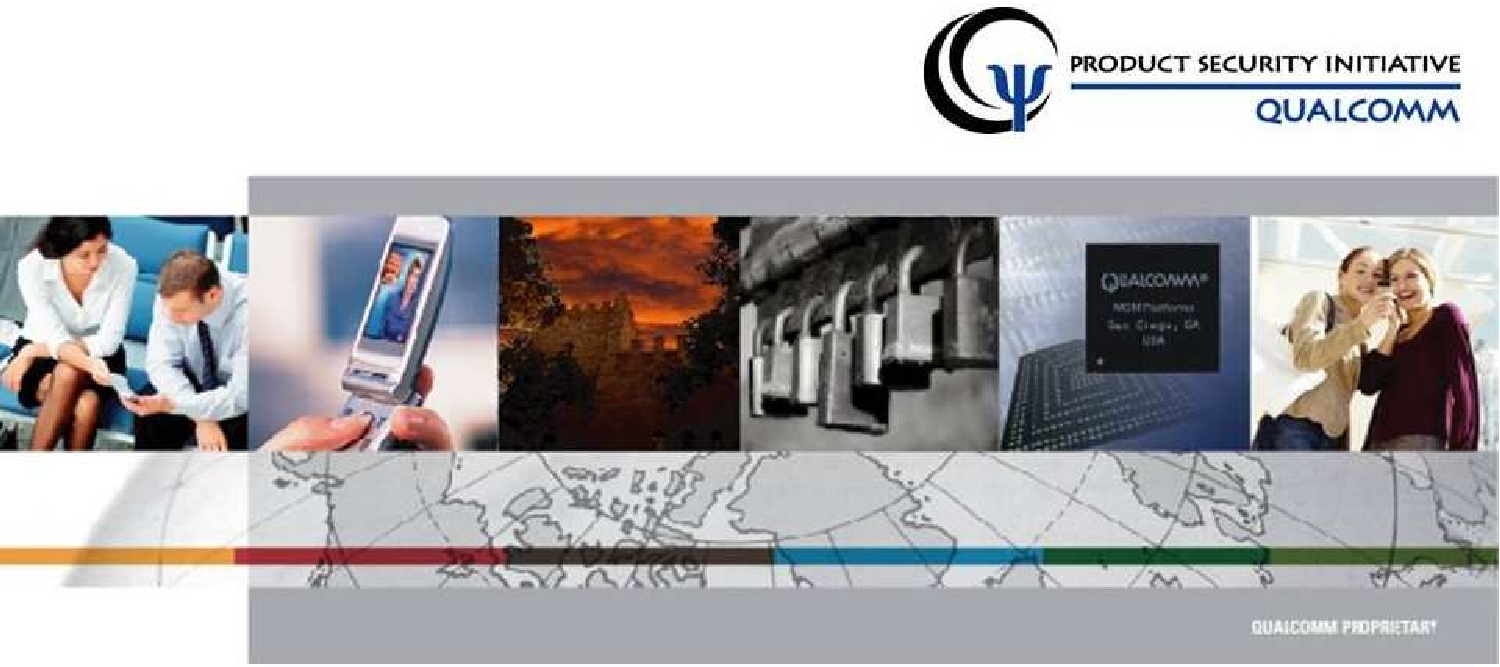
\includegraphics[width=\textwidth]{img/qpsi-cover.pdf}}
\sbox{\Cover}{}

%------------------------------------------------------------
%% Ignore page count for title page
%------------------------------------------------------------
\addtocounter{framenumber}{-1}

%------------------------------------------------------------
% Footline and headline
%------------------------------------------------------------
%% Remove footline
\setbeamertemplate{footline}{}
%% Add page number to footline
%\setbeamertemplate{footline}[page number]
\setbeamertemplate{footline}{\hfill\insertframenumber\hspace*{.5cm}}

%% Remove navigation bar
\setbeamertemplate{navigation symbols}{}

%% There is a horizontal rule at frame title
\setbeamertemplate{frametitle}
{
  \vskip 1em
  \hspace*{-0.01\textwidth}\vbox{\insertframetitle}\par 
  \HRule
}


%%%%%%%%%%%%%%%%%%%%%%%%%%%%%%%%%%%%%%%%%%%%%%%%%%%%%%%%%%%%%%%%
%% DO NOT EDIT ABOVE %% DO NOT EDIT ABOVE %% DO NOT EDIT ABOVE %
%%%%%%%%%%%%%%%%%%%%%%%%%%%%%%%%%%%%%%%%%%%%%%%%%%%%%%%%%%%%%%%%

\title[Applied Crypto Primer]
{\usebox{\Cover}\\
\mbox{\textcolor{darkred}{Applied Cryptography Primer}}
}

\author
{
Ning Shang, @syncomo on Twitter\\
}

\institute{}

\date{}

\begin{document}

\begin{frame}[plain]
\titlepage
\end{frame}

\begin{frame}{Outline}
\tableofcontents
\end{frame}

%-- Section: applied crypto --
\section{Applied Cryptography Basics}
\begin{frame}
\frametitle{Outline}
\tableofcontents[currentsection]
\end{frame}

\begin{frame}
\frametitle{Cryptography: Definition}
\emph{Cryptography} is the study of mathematics techniques related to
aspects of information security such as confidentiality, data integrity,
entity authentication, and data origin authentication. \footnote{This is
the definition of cryptography in the \emph{Handbook of Applied
Cryptography (HAC)}.}

Cryptography is not the only means of providing information security, but
rather one set of techniques.
\end{frame}

\begin{frame}
\frametitle{Goals of Cryptography}
\begin{itemize}
\item The most fundamental problem cryptography addresses: ensure 
security of communication over insecure medium.

\item Goals of cryptography: address the following areas in both
theory and practice
 \begin{itemize}
 \item Confidentiality, privacy, secrecy
 \item Data integrity
 \item Authentication
 \item Non-repudiation
 \end{itemize}
\end{itemize}
\end{frame}

\begin{frame}
\frametitle{Encoding Vs. Encryption}
\begin{itemize}
\item {\bf Encoding} is about representation of a message
\item {\bf Encryption} is about hiding a message
\end{itemize}
\end{frame}

\begin{frame}
\frametitle{A Taxonomy of Cryptographic Primitives}
\begin{figure}[!ht]
  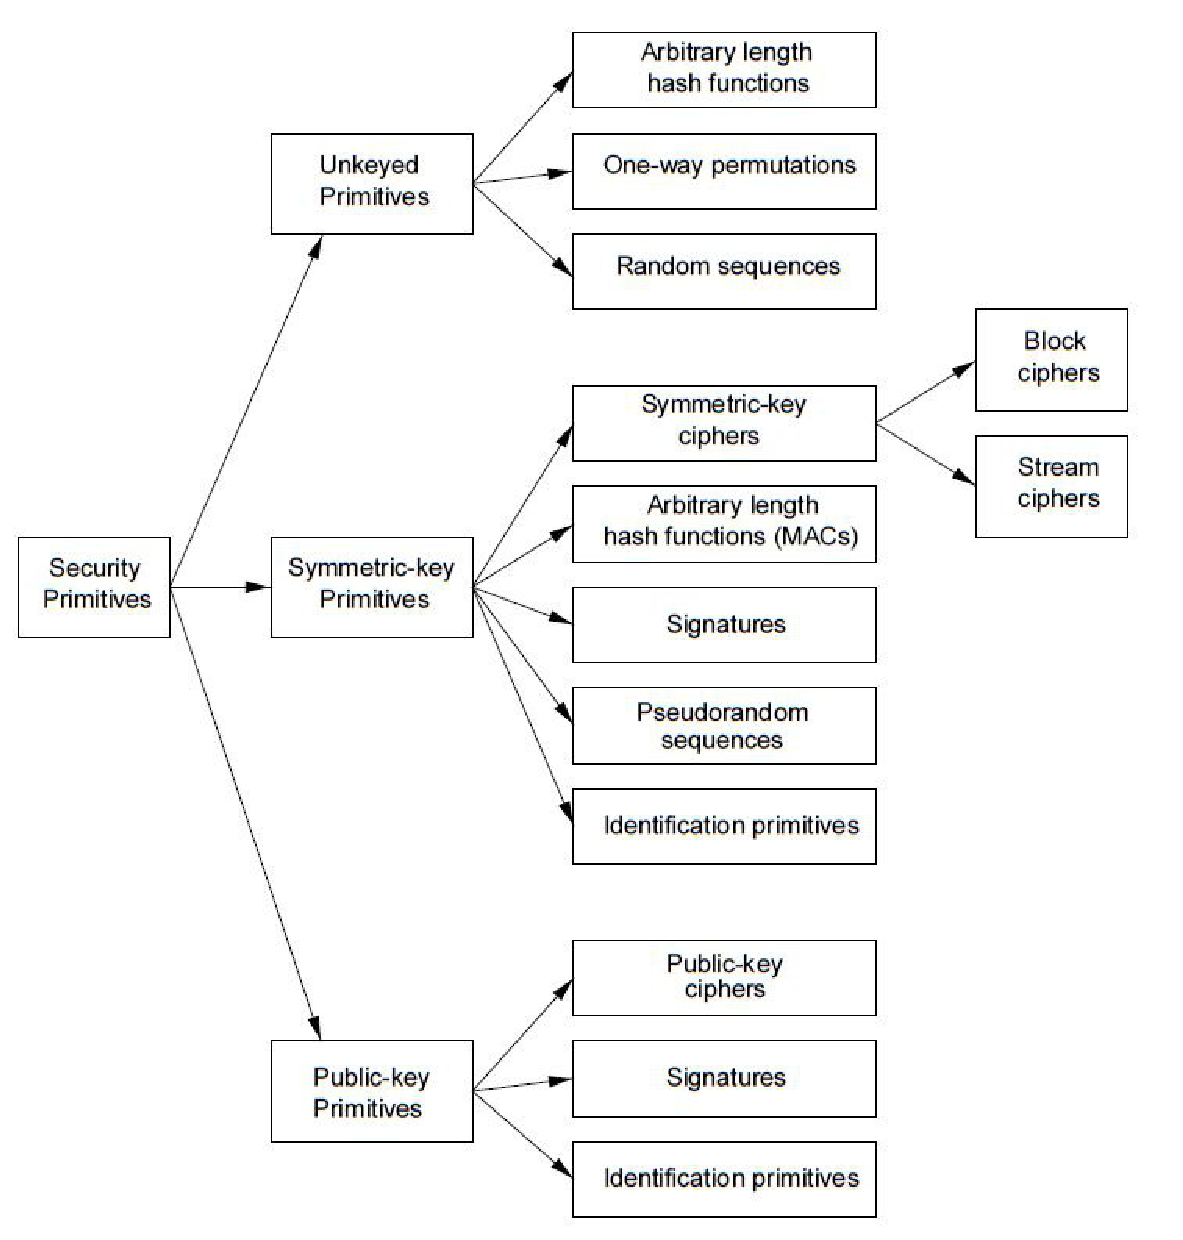
\includegraphics[width=0.5\textwidth]{fig-cryptotax.pdf}
  \caption{A taxonomy of cryptographic primitives, by the HAC}
  \label{fig:cryptotax}
\end{figure}

\end{frame}

\begin{frame}
\frametitle{Encryption}
The Figure below provides a simple model of a two-party 
communication using encryption.
\begin{figure}[!ht]
  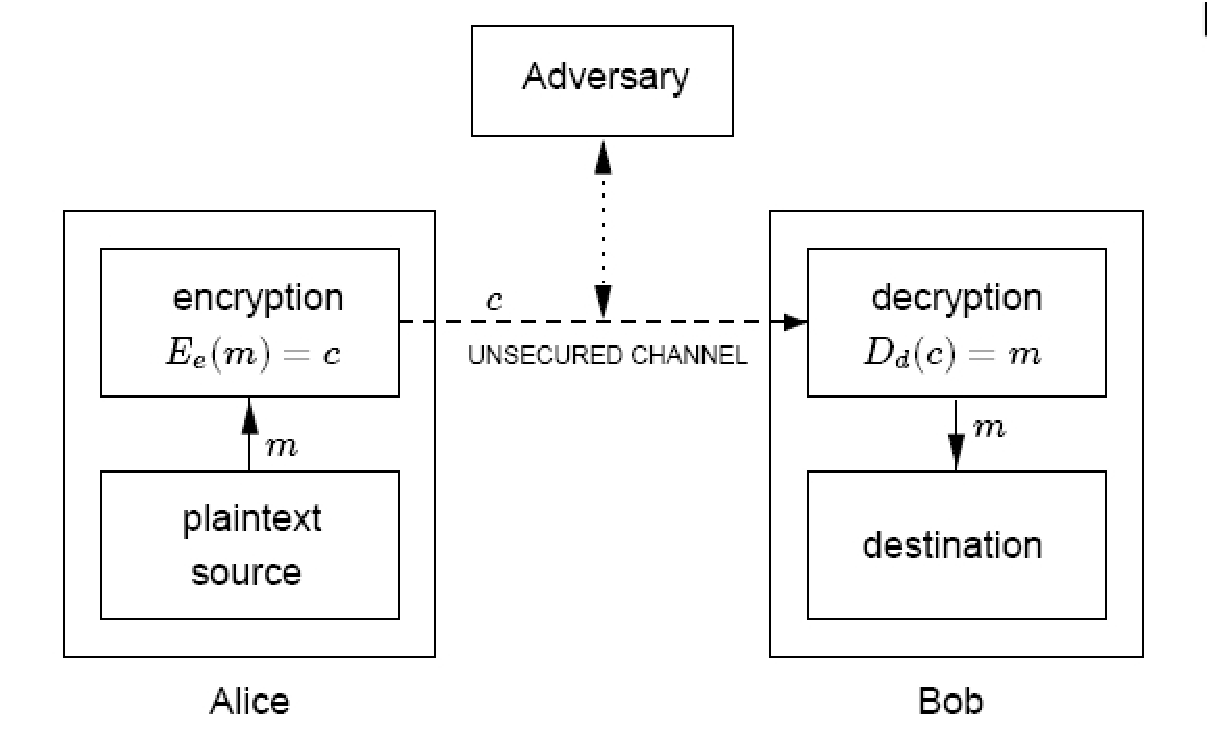
\includegraphics[width=0.4\textwidth]{fig-encryption.pdf}
  \caption{Schematic of a two-party communication using encryption}
  \label{fig:encryption}
\end{figure}

Intuitively,
\begin{itemize}
\item Symmetric (secret-key) encryption: $e = d$.
\item Asymmetric (public-key) encryption: $e \ne d$.
\end{itemize}

\end{frame}

\begin{frame}
\frametitle{Block Ciphers (Secret-Key)}
\begin{itemize}
\item Block cipher algorithms operate on a block
 \begin{itemize}
 \item DES uses 64-bit blocks, with 56-bit key
 \item AES uses 128-bit blocks, with a key of length 128, 192, or 256 bits
 \end{itemize}

\item Security of block ciphers
 \begin{itemize}
 \item When a random key is picked, the cipher should behave like a random
mapping
 \end{itemize}
\end{itemize}
\end{frame}

\begin{frame}
\frametitle{Block Cipher Modes}
\begin{itemize}
\item To encrypt a variable-length message using a block cipher, the data 
must first be divided into blocks. 
\item A block cipher mode specifies the process of encrypting each of 
these blocks. 
\end{itemize}

\begin{block}{Initialization Vector (IV)}
An IV is a (usually random) fixed-size sequence used in most of the cipher
modes
\begin{itemize}
\item IV does not need to be secret
\item IV randomizes encryption
\item IV shall not be used twice
\end{itemize}
\end{block}

\end{frame}

\begin{frame}
\frametitle{Recommendation of block cipher and modes}
General rules
\begin{itemize}
\item Use AEAD (authenticated encryption with associated data) whenever
you can
\item Consult an expert if you are unsure about the cipher or mode

\begin{figure}[hbt!]
  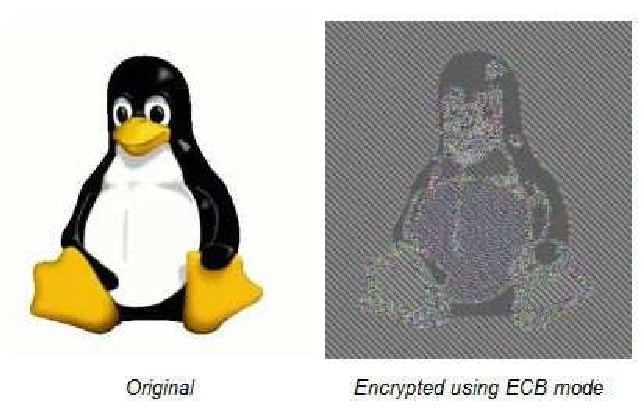
\includegraphics[width=0.3\textwidth]{fig-ecbimg.pdf}
  \caption{An image encrypted with ECB mode. 
Courtesy of ``Wikipedia::Block cipher modes of operation''.}
  \label{fig:ecbimg}
\end{figure}
\end{itemize}

\end{frame}

\begin{frame}
\frametitle{Encryption: Secret-Key Vs. Public-Key}
\begin{itemize}
\item Secret-key encryption
 \begin{itemize}
 \item Secret key exchange is usually difficult
 \item Fast
 \end{itemize}

\item Public-key encryption
 \begin{itemize}
 \item Secret key exchange is not needed
 \item Much slower than secret-key encryption algorithms
 \item Most commonly used for transport of secret keys used for bulk data
encryption by symmetric algorithms, and for encrypting small data 
items\footnote{E.g., credit card number and PINs.}
 \end{itemize}
\end{itemize}

\end{frame}

\begin{frame}
\frametitle{Achieving Data Integrity and Data Origin Authentication}
\begin{itemize}
\item Unkeyed approach: use cryptographic hash functions
 \begin{itemize}
 \item Send the hash value of a message securely
 \end{itemize}

\item Symmetric approach: use Message Authentication Code (MAC)

\item Asymmetric approach: use digital signatures
 \begin{itemize}
 \item A digital signature is a mathematical scheme for demonstrating
the authenticity of a digital message or document
 \end{itemize}
\end{itemize}
\end{frame}

\begin{frame}
\frametitle{Cryptographic Nonce and Replay Attacks}
\begin{block}{Nonce}
\begin{itemize}
\item A time-variant number that is used only once 
\item Often used in authentication protocols
\end{itemize}
\end{block}

Nonce is to ensure that old communications cannot be replayed as new.
\end{frame}

\begin{frame}
\frametitle{Key Derivation Function (KDF)}
A KDF drives one or more secret keys from a secret value. It eases
secret key management.
\begin{itemize}
\item Strech keys into longer keys
\item Convert keys into a required format
\end{itemize}

KDF examples: PBKDF2 (RFC 2898), HMAC-based Extract-and-Expand Key
Derivation Function (HKDF, RFC 5869), bcrypt, scrypt, argon2 (PHC
winner).

\end{frame}

\begin{frame}
\frametitle{Key Management}
\begin{itemize}
\item Initialization of system users within a domain
\item Generation, distribution, and provisioning of keying materials
\item Controlling the use of keying material
\item Update, revocation, and destruction of keying material
\item Storage, backup/recovery, and archival of keying material
\end{itemize}
\end{frame}

\begin{frame}
\frametitle{Key Management (Cont'd)}
Key management is the most difficult thing to get right in building a
secure system.

\begin{figure}[!ht]
  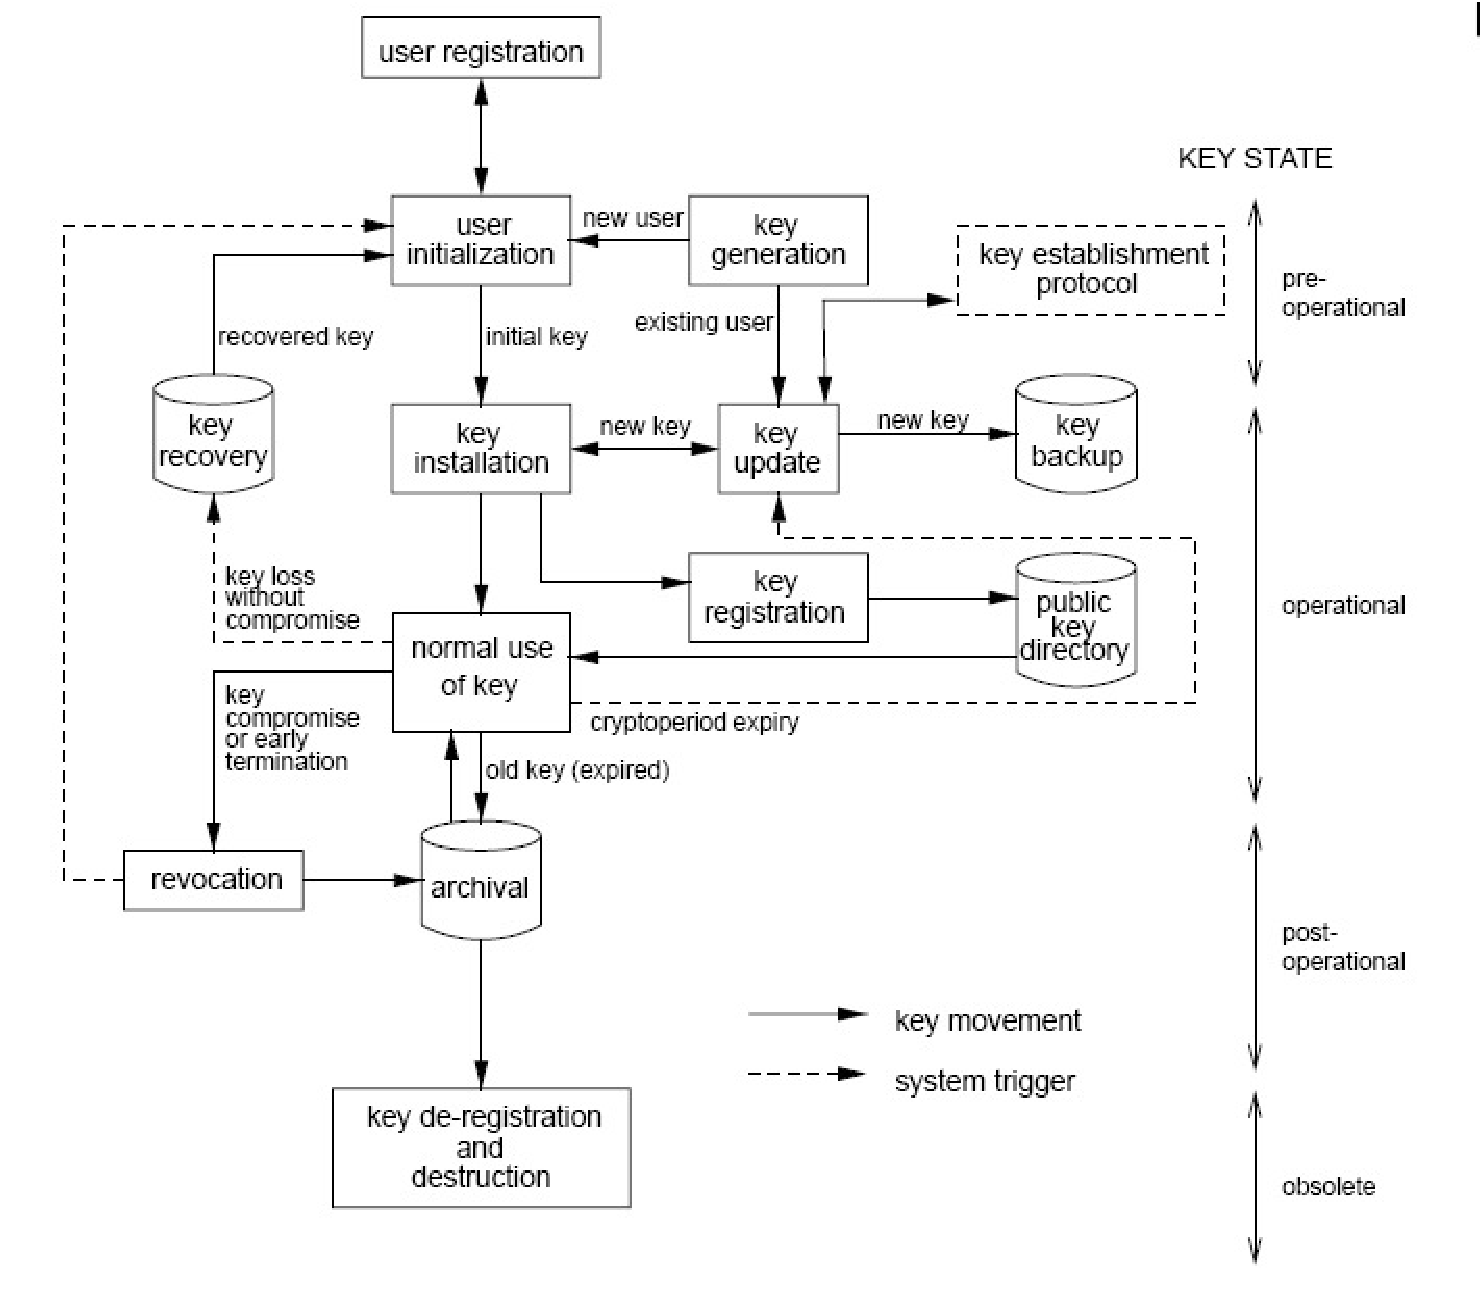
\includegraphics[width=0.5\textwidth]{fig-keymanagement.pdf}
  \caption{Key management life cycle.}
  \label{fig:keymanagement}
\end{figure}
\end{frame}


\begin{frame}
\frametitle{Key Management is Hard}
\begin{enumerate}
\item {\Huge Key management is hard}
\item {\Huge Key management is really hard}
\item {\Huge Key management is really, really hard}
%\item {\Huge Key management is really, really hard}
\end{enumerate}
\end{frame}

\begin{frame}
\frametitle{Some key management bottom lines}
\begin{itemize}
\item Stored secret keys must be secured so as to provide both 
confidentiality and authenticity
\item Stored public keys must be secured such that the authenticity is
verifiable
\item Dependencies among keying material should be avoided.
 \begin{itemize}
 \item Key management system should be able to ``fail gracefully'', i.e.,
compromise of one key does not affect others
  \begin{itemize}
  \item Oh Nine, Eff Nine: 09 F9 11 02 9D 74 E3 5B D8 41 56 C5 63 56 88 C0\\
This is an encryption key used for the DRM of HD DVDs and Blu-ray Discs,
made public on many websites.
  \end{itemize}
 \end{itemize}
\end{itemize}
\end{frame}

\begin{frame}[containsverbatim]
\frametitle{Cryptography DOs and DON'Ts}
\begin{block}{Do: Follow best practices and recommendations}
 \begin{itemize}
 \item Use well established crypto libraries; use the API correctly: ask 
for help if you do not understand something

 \item Use a strong random number generator

 \item Use standard protocols
  \begin{itemize}
  \item TLS, IPsec, OAuth
  \end{itemize}

 \item Leverage a crypto expert 
 \end{itemize}
\end{block}
\end{frame}

\begin{frame}
\frametitle{Cryptography DOs and DON'Ts (Cont'd)}
\begin{block}{Don't} 
 \begin{itemize}
 \item Don't roll your own
  \begin{itemize}
  \item Crypto design is hard, and usually error-prone
  \item Writing correct crypto code is hard
  \item If you are in doubt, ask for help
  \end{itemize}

 \item Don't use non-secure crypto algorithms for non-crypto purposes
  \begin{itemize}
  \item Use of known bad or weak algorithms hurts a company's reputation
  \end{itemize}

 \item Don't use unnecessary crypto/obfuscation
  \begin{itemize}
  \item Better to use no crypto than poorly thought-out crypto
   \begin{itemize}
   \item False sense of security to users
   \item False sense of security to developers
   \item Attackers will eventually figure out
   \item Causes confusion
   \end{itemize}
  \end{itemize}
 \end{itemize}
\end{block}
\end{frame}

%-- Section: crypto protocols --
\section{Cryptographic Protocols}
\begin{frame}
\frametitle{Outline}
\tableofcontents[currentsection]
\end{frame}
\begin{frame}
\frametitle{Entity Authentication: What Is It?}
\begin{itemize}
\item {\bf Entity Authentication:} Binding of identity to 
subject\footnote{Other names of entity authentication are 
\emph{identification} and \emph{identity verification}.}

\item Basis of entity authentication
 \begin{itemize}
 \item Something known. \\ 
 \emph{Passwords, ID numbers}
 \item Something possessed.\\ 
 \emph{National ID card, smart card}
 \item Something inherent.\\
 \emph{Biometrics, source IP, restricted area terminal}
 \end{itemize}
\end{itemize}

\end{frame}

\begin{frame}
\frametitle{Entity Authentication: How It Works}
This is how entity authentication works in general.
\begin{figure}[!ht]
  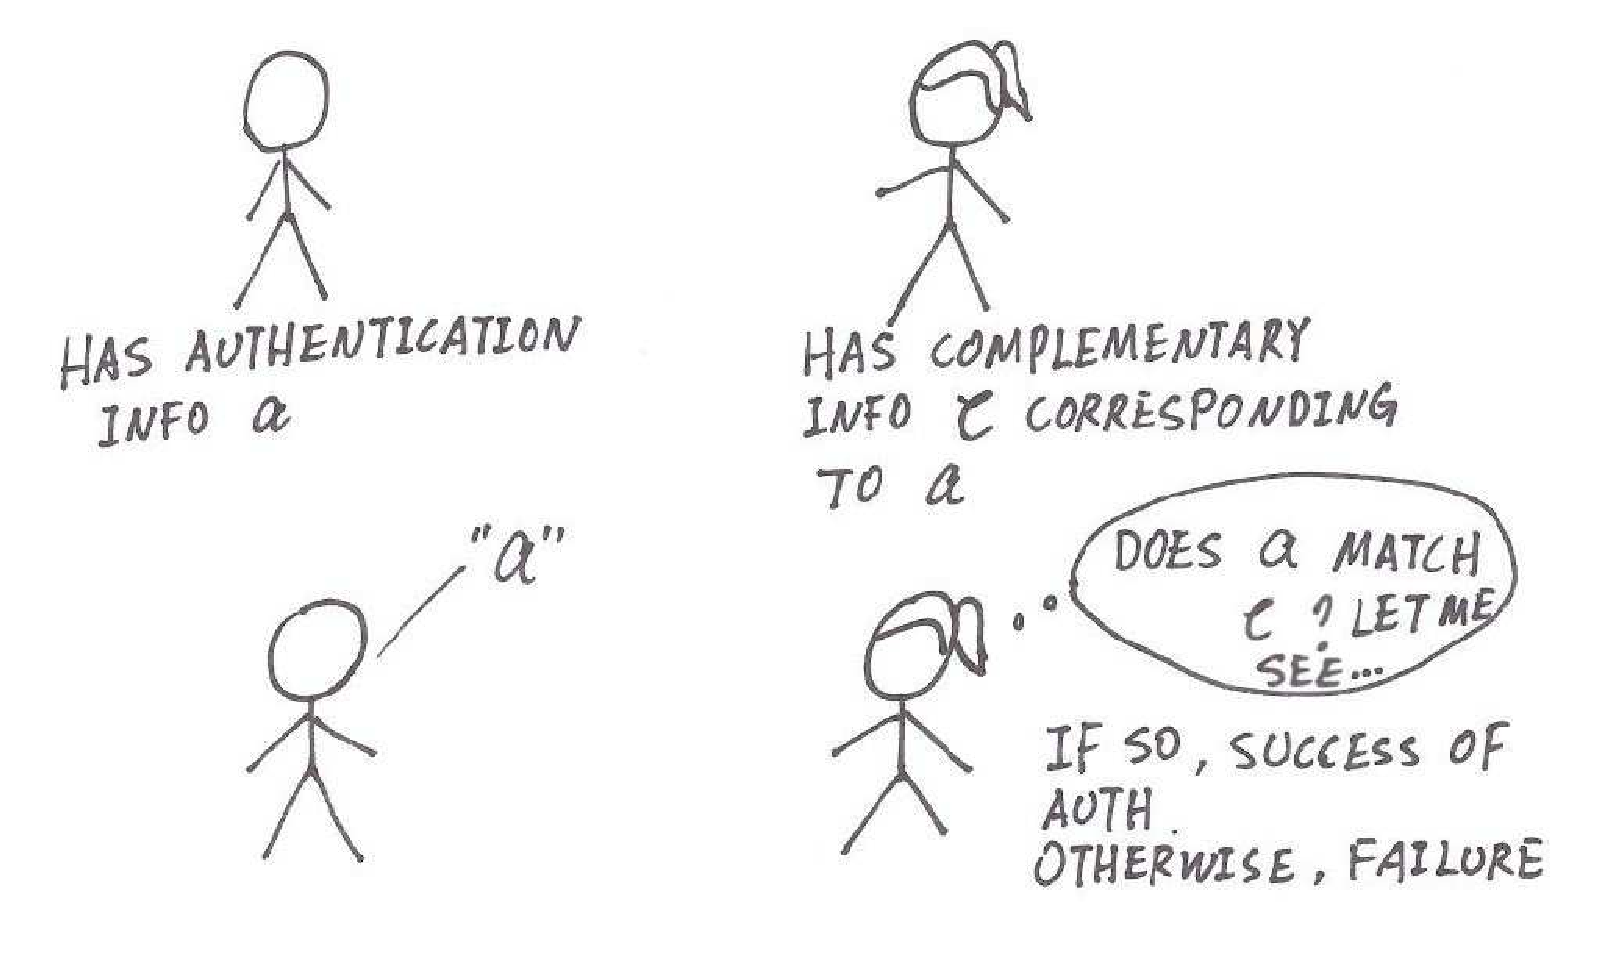
\includegraphics[width=0.7\textwidth]{fig-authentication.pdf}
  \caption{An illustration of entity authentication}
  \label{fig:authentication}
  \end{figure}

\end{frame}

\begin{frame}
\frametitle{Authentication Vs. Identity}
\begin{itemize}
\item {\bf Authentication:} binding of identity to subject
 \begin{itemize}
 \item What is \emph{identity}?
 \end{itemize}

\item {\bf Principal:} unique entity

\item {\bf Identity:} specifies a principal
\end{itemize}
\end{frame}

\begin{frame}
\frametitle{Representing Identity}
\begin{itemize}
\item Randomly chosen
\item User-chosen
\item Hierarchical: disambiguate based on levels
 \begin{itemize}
 \item File names in a file system
 \item Email addresses
  \begin{itemize}
  \item foobar@dputech.com
  \end{itemize}
 \item X.509v3: Distinguished Names
  \begin{itemize}
  \item /O=DAPU/OU=InfoSec Department/CN=shangning
  \end{itemize}
 \end{itemize}
\end{itemize}
\end{frame}

\begin{frame}
\frametitle{Validating Identity}
\begin{itemize}
\item The problem: Does identity match principal?

\item A solution: \emph{certificates}
 \begin{itemize}
 \item Certificate: Identity validated to belong to known principal
 \item Certificate Authority (CA): Certificate Issuer
 \item CA is trusted
 \end{itemize}
\end{itemize}

CA : Certificates $\sim$ Public Security Department: National ID
\end{frame}

\begin{frame}
\frametitle{Public Key Certificate}
The term \emph{certificate} refers to ``a document that attests to the 
truth of something or the ownership of something.''

\emph{A public key certificate} is a certificate attests to the
legitimate ownership of a public key and attributes a public key to a
principal.
\begin{itemize}
\item A digitally signed data structure that attests to the true ownership
of a public key
\item Identity validated to belong to a known principal
\item A principal can be 
 \begin{itemize}
 \item A person 
 \item A hardware device or 
 \item Any other entity
 \end{itemize}
\end{itemize}

\end{frame}

\begin{frame}
\frametitle{Certificate Authority}

\begin{block}{A certificate authority (or certification authority) (CA)}
\begin{itemize}
\item Issues, and possibly revokes, public key certificates 
\item Recognized and trusted by a community of users
\item Obliged to verify a certificate applicant's credentials
\end{itemize}
\end{block}

A CA is responsible for claiming \emph{``Yes, this person is who they say
they are, and we, the CA, verify that.''}
~\\
~\\
Examples of CAs that issue SSL certificates
\begin{itemize}
\item Symantec (acquired VeriSign which acquired Thawte and GeoTrust) 
\item GoDaddy 
\item GlobalSign
\item DAPU Tech can also be a CA
\end{itemize}
\end{frame}

\begin{frame}
\frametitle{Public Key Infrastructure}
\begin{itemize}
\item An infrastructure that can be used to issue, validate, and revoke 
public keys and public key certificates
\item Consists of 
 \begin{itemize}
 \item Agreed-upon standards
 \item CAs and structures among multiple CAs
 \item Methods to discover and validate certificate paths
 \item Operational and management protocols
 \item Interoperable tools
 \item Supporting legislation
 \end{itemize}
\end{itemize}
\end{frame}

\begin{frame}
\frametitle{Information Contained in a Public Key Certificate}

\begin{figure}
  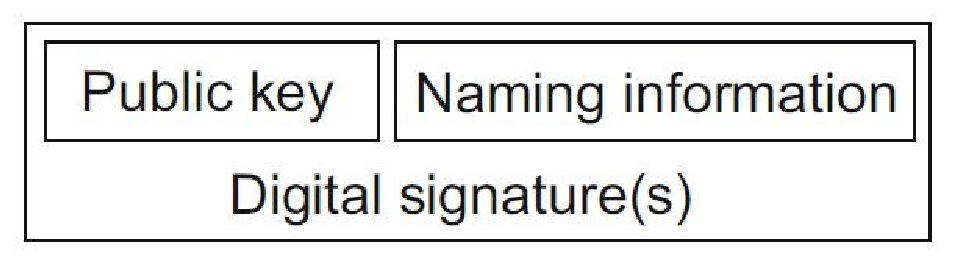
\includegraphics[width=0.5\textwidth]{fig-pkcert.pdf}
  \caption{A public key certificate comprising three pieces of information}
  \label{fig:pkcert}
\end{figure}

A public key certificate comprises at least three pieces of information
\begin{itemize}
\item A public key
\item Some naming information
 \begin{itemize}
 \item Used to identify the owner of the public key certificate
 \item Contains representation of identity
 \end{itemize}
\item One or more digital signatures
 \begin{itemize}
 \item Ties the public key and the naming information together
 \end{itemize}
\end{itemize}
\end{frame}

\begin{frame}
\frametitle{X.509 Hierarchical Trust Model}
X.509 hierarchical trust model
\begin{figure}
  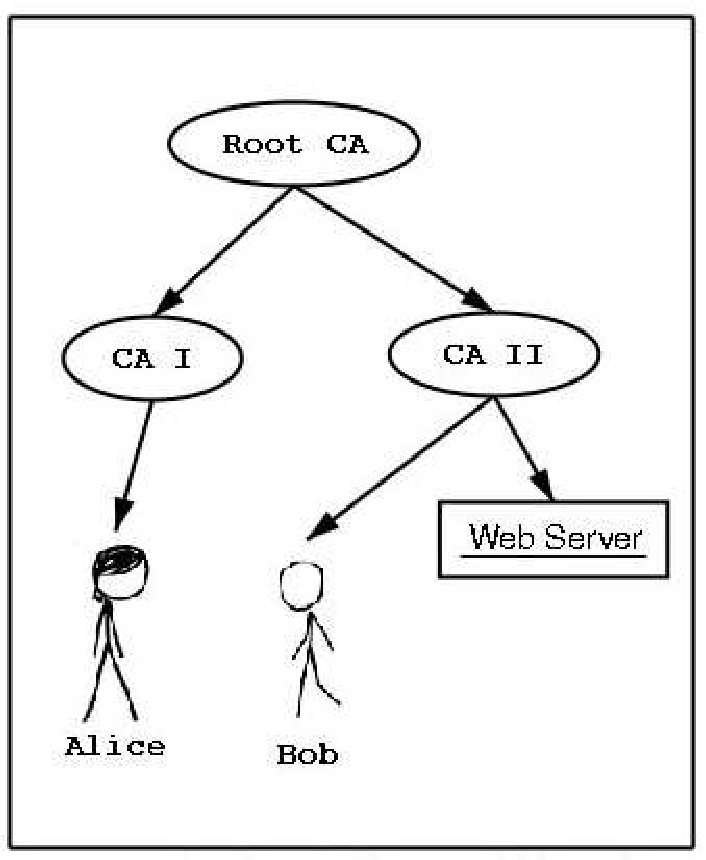
\includegraphics[width=0.4\textwidth]{fig-x509trust.pdf}
  \caption{X.509 certificate chains}
  \label{fig:x509trust}
\end{figure}
\end{frame}

\begin{frame}
\frametitle{Trust Model in TLS and SSL}
\begin{itemize}
\item As of today, the X.509 trust model is prevailing.
\end{itemize}
\end{frame}

\begin{frame}
\frametitle{What are SSL and TLS?}
\begin{itemize}
\item Protocols that provide end-to-end communication security over the 
Internet.
 \begin{itemize}
 \item Confidentiality
 \item Data integrity
 \item Data origin authentication
 \item Entity authentication
 \end{itemize}

\item {\bf SSL:} Secure Socket Layer
 \begin{itemize}
 \item Originally developed by Netscape in 1995 to provide secure and 
authenticated connections between browsers and servers
 \end{itemize}

\item {\bf TLS:} Transport Layer Security
 \begin{itemize}
 \item IETF made SSLv3 an open standard in 1999, and called it TLSv1
 \end{itemize}
\end{itemize}

The latest TLS version is 1.3 (draft as of May 2017)

\begin{block}{}
\begin{itemize}
\item There are security vulnerabilities in SSLv1 and SSLv2
\item Use the latest available TSL version in product
\item Do not use broken ciphers in SSL/TLS
\end{itemize}
\end{block}
\end{frame}

\begin{frame}
\frametitle{SSL/TLS Features}
\begin{itemize}
\item Two types of functions
 \begin{itemize}
 \item Establish a secure connection between communicating parties
 \item Use this connection to securely transmit higher layer protocol
data from the sender to the recipient
 \end{itemize}

\item Either server-only authentication or server-client authentication
is allowed
 \begin{itemize}
 \item Server-only authentication: server sends certificate
 \item Server-client authentication: client sends certificate as well
 \end{itemize}

\item SSL is not a single protocol: it is composed of a few subprotocols in
two sublayers
\end{itemize}
\end{frame}


\begin{frame}
\frametitle{SSL/TLS Connections and SSL Sessions}
\begin{itemize}
\item {\bf SSL connection}
 \begin{itemize}
 \item A one-time transport of information between two peers
 \item Connections are transient
 \item Every connection is associated with a \emph{session}
 \end{itemize}

\item {\bf SSL session}
 \begin{itemize}
 \item A session is created by the SSL handshaking protocol
 \item Multiple connections can exist in one session
 \item A session is characterized by a set of security parameters that
apply to all the connections in the session
 \item The concept of a session eliminates the need for negotiating the 
security parameters for each separate connection
 \end{itemize}
\end{itemize}
\end{frame}

\begin{frame}[containsverbatim]
\frametitle{SSL/TLS Implementations}
\begin{itemize}
\item OpenSSL (BSD)
\item BoringSSL (Google's fork of OpenSSL)
\item GnuTLS (LGPL)
\item SChannel (Microsoft)
\item SharkSSL, mbedTLS (for embedded devices)
\item Etc.
\end{itemize}
\end{frame}


%-- References --
%\begin{frame}[allowframebreaks]{References}
%\tiny
%\bibliographystyle{unsrt}
%\bibliography{ref}
%\end{frame}
\end{document}
